\documentclass[11pt,a4paper]{article}

% ---------- packages ----------
\usepackage[utf8]{inputenc}
\usepackage[T1]{fontenc}
\usepackage[margin=2.2cm]{geometry}
\usepackage{xcolor}
\usepackage{amssymb}
\usepackage{booktabs}
\usepackage{enumitem}
\usepackage{tikz}
\usetikzlibrary{arrows.meta,positioning,calc,shapes.geometric,backgrounds,fit}
\usepackage[colorlinks=true,linkcolor=blue!50!black,urlcolor=blue!50!black]{hyperref}

% ---------- colours ----------
\definecolor{coldblue}{RGB}{30,120,200}
\definecolor{hotred}{RGB}{200,50,40}
\definecolor{metal}{RGB}{150,150,160}
\definecolor{boxblue}{RGB}{225,238,250}
\definecolor{boxgreen}{RGB}{225,245,228}
\definecolor{boxorange}{RGB}{252,237,213}

% ---------- styles ----------
\tikzset{
  block/.style={draw,rounded corners,minimum width=2.7cm,minimum height=1.1cm,align=center,font=\small,fill=boxblue},
  sens/.style ={draw,rounded corners,minimum width=2.7cm,minimum height=1.1cm,align=center,font=\small,fill=boxgreen},
  st/.style   ={draw,rounded corners,minimum width=1.9cm,minimum height=0.9cm,align=center,font=\scriptsize,fill=boxorange},
  flow/.style ={-{Latex[length=2.5mm]},thick},
  lbl/.style  ={font=\scriptsize,fill=white,inner sep=1pt,align=center}
}

\newsavebox{\gbbox}
\newenvironment{checkbox}[1]
  {\par\medskip\noindent\begin{lrbox}{\gbbox}\begin{minipage}{0.95\linewidth}\footnotesize\textbf{#1}\par\smallskip}
  {\end{minipage}\end{lrbox}\setlength{\fboxsep}{8pt}\fcolorbox{red!60!black}{red!5}{\usebox{\gbbox}}\par\medskip}
\newenvironment{tipbox}[1]
  {\par\medskip\noindent\begin{lrbox}{\gbbox}\begin{minipage}{0.95\linewidth}\footnotesize\textbf{#1}\par\smallskip}
  {\end{minipage}\end{lrbox}\setlength{\fboxsep}{8pt}\fcolorbox{green!45!black}{green!5}{\usebox{\gbbox}}\par\medskip}

\newcommand{\warn}{\textcolor{orange!80!black}{$\triangle$}}

\title{\vspace{-1.5cm}\textbf{The Real Two-Rail Robot}\\[3pt]
\large Build \& system guide for the actual rail-guided, self-watering\\[2pt]
\large PV-cleaning robot --- the deployment machine, not the bench}
\author{Graduation Project --- prototype phase}
\date{17 June 2026}

\begin{document}
\maketitle
\vspace{-0.5cm}

\noindent\fbox{\parbox{0.98\linewidth}{\small
\textbf{What this guide is.} The bench guide (\texttt{guide.pdf}) builds a small moving cart on a table to
prove the motion. \emph{This} guide describes the \textbf{real robot} --- the one that climbs a tilted
solar panel on two rails, cleans the glass with a full-width brush, and makes its own washing water from
the air. The numbers here come from the frozen design files: \texttt{MARKET\_PARTS\_BUYLIST.md},
\texttt{CAD\_DESIGN\_PACKAGE}, \texttt{ELECTRICAL\_DESIGN}, and \texttt{ROS2\_ARCHITECTURE}.}}

\tableofcontents

% ============================================================
\section{The whole machine at a glance}

The robot is a \textbf{gantry on two rails}. The rails run straight up the slope of a solar panel
(tilted about $24^{\circ}$). The carriage spans both rails and carries a brush as wide as the panel.
It drives \emph{up} the glass and back \emph{down}, sweeping dust off in straight ``fall-line'' passes.
It does not make its own water while moving --- a \textbf{stationary dock} at the bottom of the rails
makes distilled water from the air using cooling chips, and the robot tops up its tank there.

\begin{figure}[h]
\centering
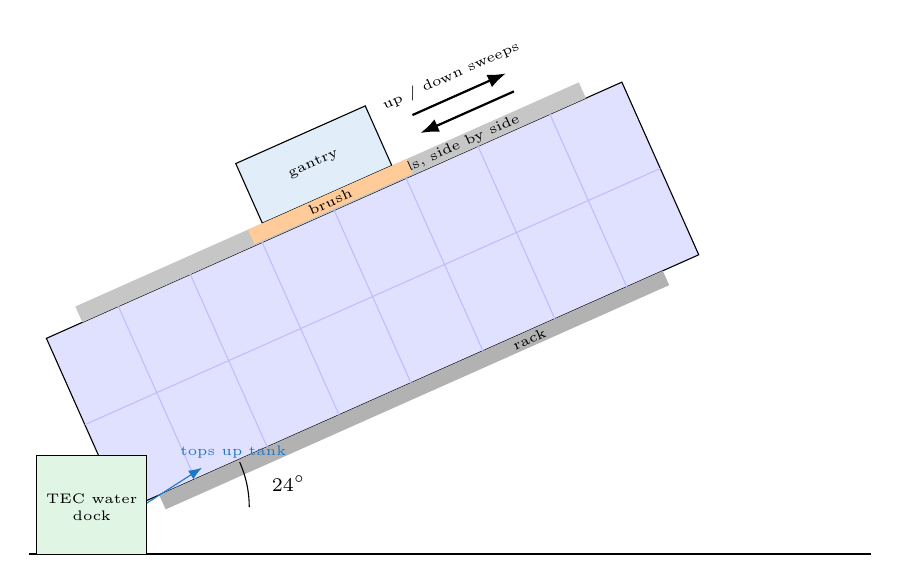
\begin{tikzpicture}[scale=1]
% ground
\draw[thick] (-1.2,-0.55)--(9.5,-0.55);
\begin{scope}[rotate=24]
  % panel
  \fill[blue!12] (0,0) rectangle (8,2.4); \draw (0,0) rectangle (8,2.4);
  \foreach \x in {1,2,...,7}{\draw[blue!25] (\x,0)--(\x,2.4);}
  \draw[blue!25] (0,1.2)--(8,1.2);
  % rails on the surface
  \fill[gray!45] (0.5,2.4) rectangle (7.5,2.62);
  \node[font=\tiny,rotate=24] at (5.6,2.51){2 rails, side by side};
  % rack strip on the panel edge
  \fill[gray!60] (0.5,-0.2) rectangle (7.5,0);
  \node[font=\tiny,rotate=24] at (5.6,-0.1){rack};
  % carriage
  \fill[boxblue] (3.1,2.62) rectangle (4.9,3.45); \draw (3.1,2.62) rectangle (4.9,3.45);
  \node[font=\tiny,align=center,rotate=24] at (4.0,3.05){gantry};
  % brush
  \fill[orange!40] (2.9,2.42) rectangle (5.1,2.62);
  \node[font=\tiny,rotate=24] at (4.0,2.52){brush};
  % sweep arrows
  \draw[-{Latex},thick] (5.4,3.1)--(6.7,3.1);
  \draw[{Latex}-,thick] (5.4,2.85)--(6.7,2.85);
  \node[font=\tiny,rotate=24] at (6.05,3.35){up / down sweeps};
\end{scope}
% tilt angle
\draw (1.6,0.05) arc (0:24:1.4); \node[font=\scriptsize] at (2.1,0.35){$24^{\circ}$};
% dock
\fill[boxgreen] (-1.1,-0.55) rectangle (0.3,0.7); \draw (-1.1,-0.55) rectangle (0.3,0.7);
\node[font=\tiny,align=center] at (-0.4,0.05){TEC water\\dock};
\draw[-{Latex},coldblue] (0.3,0.1)--(1.0,0.55); \node[font=\tiny,coldblue,right] at (0.6,0.75){tops up tank};
\end{tikzpicture}
\caption{Side view. Two rails run up a $24^{\circ}$ panel; the gantry carriage rides them with a
full-width brush and sweeps up and down. A stationary dock at the foot of the rails harvests water and
refills the robot's tank.}
\end{figure}

\begin{tipbox}{How it differs from your bench}
The bench proves \emph{one} thing: a cart moves itself along a rail. The real robot adds four things the
bench leaves out --- it \textbf{climbs a $24^{\circ}$ slope} (so it needs a rack-and-pinion, not a belt),
it carries a \textbf{full-width brush}, it has a \textbf{second brain} (a Raspberry Pi) for autonomy, and
its water comes from a \textbf{separate dock}, not the carriage.
\end{tipbox}

% ============================================================
\section{The two rails on the panel}

Two lengths of \textbf{2040 V-slot rail}, each about \textbf{2.4 m}, are fixed up the long edges of the
panel, parallel, the gantry's width apart. They are the tracks the carriage rolls on and the backbone
that holds it square on the glass. Alongside one rail runs a toothed \textbf{rack} strip --- that is what
the robot's gear teeth bite into to climb (next section).

\begin{itemize}[leftmargin=*,itemsep=1pt]
  \item Same height, exactly parallel --- measure the gap at top and bottom, they must match.
  \item Fixed to the panel frame with L-brackets and T-nuts (never drilled into the glass).
  \item End stops / limit switches at the top and bottom so the carriage knows where the travel ends.
\end{itemize}

% ============================================================
\section{The drive: rack-and-pinion, not wheels}

This is the single biggest change from the bench. On a $24^{\circ}$ sheet of glass, plain rubber wheels
\textbf{cannot grip hard enough to climb} --- the simulation confirmed they slip even with very sticky
tyres. The fix is a \textbf{rack-and-pinion}: a fixed toothed strip (the rack) and a toothed gear (the
pinion) on the motor. The teeth mesh, so the drive is \emph{positive} --- it cannot slip.

\begin{figure}[h]
\centering
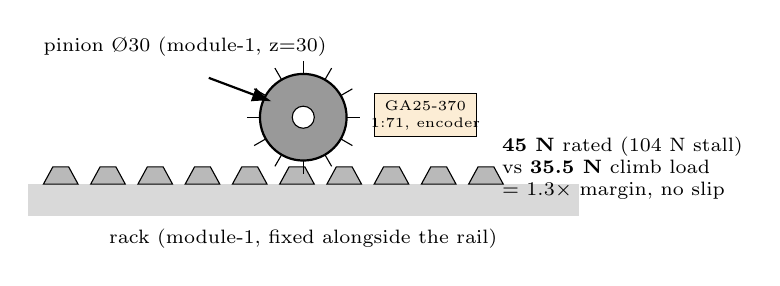
\begin{tikzpicture}[scale=1]
% rack
\fill[gray!30] (0,0) rectangle (7,0.4);
\foreach \x in {0.2,0.8,...,6.2}{\draw[fill=gray!55] (\x,0.4)--(\x+0.12,0.62)--(\x+0.32,0.62)--(\x+0.44,0.4)--cycle;}
\node[font=\scriptsize,below] at (3.5,-0.05){rack (module-1, fixed alongside the rail)};
% pinion
\draw[thick,fill=gray!80] (3.5,1.25) circle (0.55);
\foreach \a in {0,30,...,330}{\draw[fill=gray!60] (3.5,1.25)++(\a:0.55)--++(\a:0.17);}
\draw[fill=white] (3.5,1.25) circle (0.14);
\node[font=\scriptsize,above] at (2.0,1.9){pinion \O30 (module-1, z=30)};
\draw[flow] (2.3,1.75)--(3.1,1.45);
% motor
\fill[boxorange] (4.4,1.0) rectangle (5.7,1.55); \draw (4.4,1.0) rectangle (5.7,1.55);
\node[font=\tiny,align=center] at (5.05,1.27){GA25-370\\1:71, encoder};
% force note
\node[font=\scriptsize,align=left,right] at (5.9,0.6){\textbf{45 N} rated (104 N stall)\\vs \textbf{35.5 N} climb load\\$=$ 1.3$\times$ margin, no slip};
\end{tikzpicture}
\caption{Rack-and-pinion drive. The pinion's teeth mesh into the fixed rack, so climbing force comes from
gear teeth, not from friction. Two driven rails share the load; each GA25-370 gearmotor has a 1.86$\times$
torque margin.}
\end{figure}

\textbf{Two driven rails.} Each rail gets its own GA25-370 12\,V 1:71 gearmotor (the same family as your
bench motor, just the slower 60\,rpm ratio) turning a \O30 pinion. Together they give a comfortable
margin to climb the 35.5\,N slope load.

\begin{checkbox}{\warn\ The carriage must not slide back when the motor stops}
A GA25-370 gearbox is \emph{not} self-locking, so on the tilt the carriage would creep down when power is
cut. The design holds it two ways together: the \textbf{Cytron MDD3A driver's brake mode} (it shorts the
motor windings at rest) plus a small \textbf{sprung detent} that drops into the rack at the park spot. If
you want a purely mechanical hold instead, swap to a \textbf{JGY-370 worm gearmotor}, which is
self-locking by nature (it trades some speed and efficiency).
\end{checkbox}

\noindent The rack and pinion are \textbf{module-1} steel and have no local supplier --- they are the one
mechanically-critical \textbf{import} (Aliexpress, 2--4 weeks). Confirm the pinion bore matches the GA25
shaft before ordering, or buy a shaft adapter locally.

% ============================================================
\section{The gantry carriage}

Looking straight up the slope, the carriage is a \textbf{cross-beam} (~0.92\,m) bridging the two rails.
Each end rides the rail on V-wheels and carries a driven pinion. Slung under the beam is the full-width
brush, the spray bar, the water tank, the battery, and the electronics.

\begin{figure}[h]
\centering
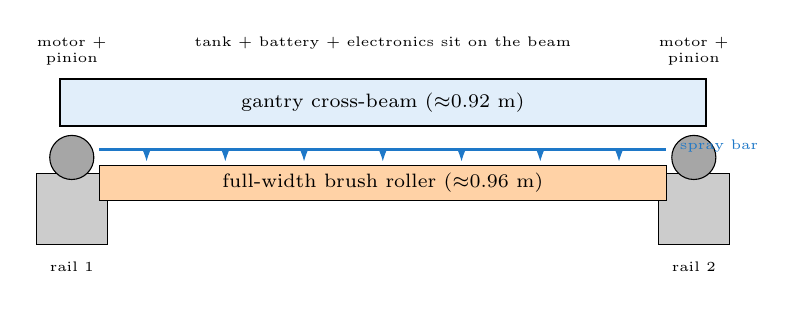
\begin{tikzpicture}[scale=1]
% rails (cross-sections)
\fill[gray!40] (-0.4,0) rectangle (0.5,0.9); \draw(-0.4,0) rectangle (0.5,0.9);
\node[font=\tiny,below] at (0.05,-0.1){rail 1};
\fill[gray!40] (7.5,0) rectangle (8.4,0.9); \draw(7.5,0) rectangle (8.4,0.9);
\node[font=\tiny,below] at (7.95,-0.1){rail 2};
% gantry beam
\fill[boxblue] (-0.1,1.5) rectangle (8.1,2.1); \draw[thick] (-0.1,1.5) rectangle (8.1,2.1);
\node[font=\scriptsize] at (4.0,1.8){gantry cross-beam ($\approx$0.92 m)};
% pinions+motors at each end
\draw[fill=gray!70] (0.05,1.1) circle (0.28); \draw[fill=gray!70] (7.95,1.1) circle (0.28);
\node[font=\tiny,align=center] at (0.05,2.45){motor +\\pinion}; \node[font=\tiny,align=center] at (7.95,2.45){motor +\\pinion};
% brush
\fill[orange!35] (0.4,0.55) rectangle (7.6,1.0); \draw (0.4,0.55) rectangle (7.6,1.0);
\node[font=\scriptsize] at (4.0,0.78){full-width brush roller ($\approx$0.96 m)};
% spray bar
\draw[very thick,coldblue] (0.4,1.2)--(7.6,1.2);
\foreach \x in {1,2,...,7}{\draw[-{Latex},coldblue] (\x,1.2)--(\x,1.05);}
\node[font=\tiny,coldblue,right] at (7.65,1.25){spray bar};
% payload note
\node[font=\tiny,align=center,fill=white] at (4.0,2.55){tank + battery + electronics sit on the beam};
\end{tikzpicture}
\caption{Front view, looking up the slope. The cross-beam spans both rails; each end is driven by its own
motor + pinion. The brush, spray bar, tank, battery and electronics hang on the beam. Total mass closes
at about 8\,kg.}
\end{figure}

% ============================================================
\section{Cleaning head: full-width brush + spray}

\begin{itemize}[leftmargin=*,itemsep=1pt]
  \item \textbf{Brush:} a $\approx$0.96\,m roller, $\approx$\O50\,mm, microfibre over a PVC/aluminium
  core, on two 608-class bearings, spun by its own GA25-370 ($\approx$100\,rpm) and switched by an
  \textbf{IRLZ44N} logic-level MOSFET.
  \item \textbf{Spray:} a 12\,V diaphragm pump feeds a 0.96\,m spray bar with about nine flat-fan nozzles.
  The dose is light --- \textbf{0.3\,L/m\textsuperscript{2}} (a microfibre wash, not a flood), so a whole
  panel needs only $\approx$0.6\,L. Pump switched by a second IRLZ44N.
\end{itemize}

\noindent Wetting a thin film, then wiping with microfibre, removes dust without a heavy water bill ---
that low dose is what makes self-supply from the air feasible.

% ============================================================
\section{Water from the air: the TEC dock}

The water maker is a \textbf{stationary dock}, not on the carriage (keeping it off the carriage is what
lets the mass close at 8\,kg). It pulls humid air across cold surfaces; water condenses, drips, and
collects in a tank the robot refills from.

\begin{figure}[h]
\centering
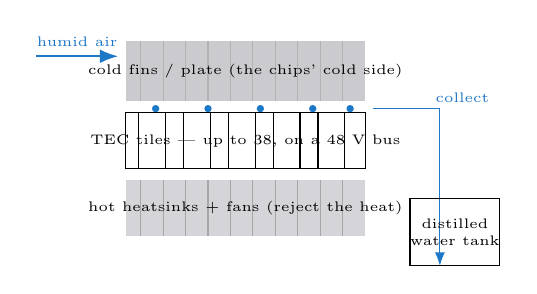
\begin{tikzpicture}[scale=0.95]
% humid air in
\draw[-{Latex},coldblue,thick] (-1.0,3.0)--(0.1,3.0); \node[font=\tiny,coldblue,above] at (-0.45,3.0){humid air};
% cold fins
\fill[metal!50] (0.2,2.4) rectangle (3.4,3.2); \foreach \x in {0.4,0.7,...,3.2}{\draw[gray!60](\x,2.4)--(\x,3.2);}
\node[font=\tiny] at (1.8,2.8){cold fins / plate (the chips' cold side)};
% droplets
\foreach \x in {0.6,1.3,2.0,2.7,3.2}{\fill[coldblue] (\x,2.3) circle (1.4pt);}
% TEC tiles
\fill[white] (0.2,1.5) rectangle (3.4,2.25); \draw (0.2,1.5) rectangle (3.4,2.25);
\foreach \x in {0.55,1.15,1.75,2.35,2.95}{\draw (\x-0.18,1.5) rectangle (\x+0.18,2.25);}
\node[font=\tiny] at (1.8,1.87){TEC tiles --- up to 38, on a 48 V bus};
% hot heatsinks + fans
\fill[metal!40] (0.2,0.6) rectangle (3.4,1.35); \foreach \x in {0.4,0.7,...,3.2}{\draw[gray!70](\x,0.6)--(\x,1.35);}
\node[font=\tiny] at (1.8,0.97){hot heatsinks + fans (reject the heat)};
% collection to tank
\draw[-{Latex},coldblue] (3.5,2.3)--(4.4,2.3)--(4.4,0.2);
\draw (4.0,0.2) rectangle (5.2,1.1); \node[font=\tiny,align=center] at (4.6,0.65){distilled\\water tank};
\node[font=\tiny,coldblue] at (4.7,2.45){collect};
\end{tikzpicture}
\caption{The dock. Cooling chips chill a finned plate; humid air condenses on it and drips into a tank.
The hot side is dumped by heatsinks and fans. At full residential scale 38 tiles run on a 48\,V bus
(raising the bus from 12\,V to 48\,V cuts the current from 228\,A to 63\,A).}
\end{figure}

\begin{tipbox}{Same physics as your bench harvest test}
This is exactly the cold-plate / hot-heatsink stack from the bench guide, just many tiles instead of
four, and switched in strings by 100\,V \textbf{IRLB4030} MOSFETs on a 48\,V bus instead of a single
12\,V supply. Prove it on four tiles first.
\end{tipbox}

% ============================================================
\section{Power}

\begin{itemize}[leftmargin=*,itemsep=1pt]
  \item \textbf{On the carriage:} a \textbf{12\,V 10\,Ah LiFePO\textsubscript{4}} battery ($\approx$1.3\,kg),
  good for about five cleaning sessions, topped up at the dock. A small \textbf{LM2596} buck makes the
  5\,V logic rail (just like your bench).
  \item \textbf{At the dock:} the cooling tiles run on a \textbf{48\,V} bus. Off-grid, that needs PV +
  one 48\,V MPPT (EPever Tracer4215AN) + a battery bank. \textbf{Recommended: grid-couple it} --- if the
  house already has a PV array, the dock draws its night load from the house and you skip the dedicated
  PV/MPPT/battery, leaving only $\approx$14,000\,EGP of marginal water-making hardware.
\end{itemize}

% ============================================================
\section{Brains \& autonomy}

The real robot has \textbf{two} brains. The ESP32 (which you already know) handles the fast, real-time
jobs --- motor PWM, reading encoders, the cooling set-point. A \textbf{Raspberry Pi 4} sits above it
running ROS\,2, doing the planning and the overall sequence. They talk over a USB serial link
(``micro-ROS''). There is \textbf{no camera/SLAM}: the robot knows where it is from the wheel encoders
plus an IMU, re-zeroing on the end-of-travel switch each pass.

\begin{figure}[h]
\centering
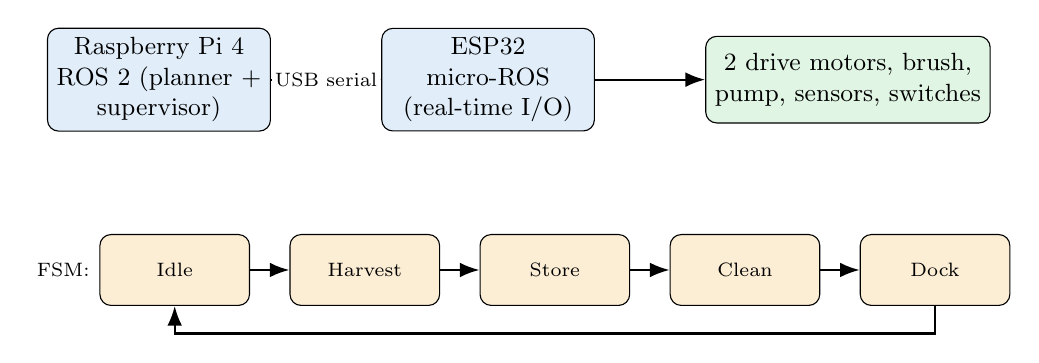
\begin{tikzpicture}[node distance=0.8cm and 1.4cm]
\node[block](pi){Raspberry Pi 4\\ROS 2 (planner +\\supervisor)};
\node[block,right=of pi](esp){ESP32\\micro-ROS\\(real-time I/O)};
\node[sens,right=of esp](io){2 drive motors, brush,\\pump, sensors, switches};
\draw[flow] (pi)--node[lbl]{USB serial}(esp);
\draw[flow] (esp)--(io);
% FSM chain
\node[st,below=1.3cm of pi.south,xshift=0.2cm](idle){Idle};
\node[st,right=0.5cm of idle](harv){Harvest};
\node[st,right=0.5cm of harv](store){Store};
\node[st,right=0.5cm of store](clean){Clean};
\node[st,right=0.5cm of clean](dock){Dock};
\draw[flow](idle)--(harv); \draw[flow](harv)--(store); \draw[flow](store)--(clean);
\draw[flow](clean)--(dock); \draw[flow](dock.south)--++(0,-0.35)-|(idle.south);
\node[font=\scriptsize,left] at (idle.west){FSM:};
\end{tikzpicture}
\caption{Two-brain control. The Pi plans and runs the state machine (Idle $\to$ Harvest water $\to$ Store
$\to$ Clean the panel $\to$ Dock and recharge); the ESP32 does the hard-real-time motor and sensor work.}
\end{figure}

\noindent\textbf{Sensors:} DHT22 (air temperature/humidity for dew point), DS18B20 (cold-plate
temperature), INA219 or ACS712 (current/power), MPU-6050 (tilt and fall trip), two limit switches
(end-of-travel), and the encoders built into the drive motors.

% ============================================================
\section{Build order (recommended)}

\begin{enumerate}[leftmargin=*,itemsep=2pt]
  \item Mount the two rails on the panel frame, parallel, with the rack alongside one rail.
  \item Build the gantry cross-beam; fit V-wheels and a driven motor + pinion at each end.
  \item Set the carriage on the rails; check it rolls and that both pinions mesh the rack cleanly.
  \item Wire the two drive motors to the MDD3A; test the climb up and down, with brake-hold at rest.
  \item Add the brush roller + its motor, then the spray bar, pump, and tank.
  \item Build the stationary TEC dock and prove water harvest on a few tiles first, then scale up.
  \item Add the ESP32, then the Raspberry Pi; bring up the encoder/IMU odometry and the limit-switch
  re-zero.
  \item Bring the supervisor state machine online and run a full Idle $\to$ Dock cycle.
\end{enumerate}

\begin{tipbox}{Build it bottom-up}
Every block above is testable on its own. Get the climb working before the brush, the brush before the
water, the water before the autonomy. The bench you are building now is step~3--4 in miniature.
\end{tipbox}

% ============================================================
\section{Parts \& sourcing}

The full priced bill of materials --- every part, vendor, link, and quantity for both the bench and the
full residential dock --- is in \texttt{MARKET\_PARTS\_BUYLIST.md}. Headlines:

\begin{itemize}[leftmargin=*,itemsep=1pt]
  \item \textbf{Buy in Cairo:} rails, V-wheels, brackets, T-nuts, GA25-370 motors, Cytron MDD3A, MOSFETs,
  bearings, TEC tiles, sensors, ESP32, pump, limit switches (Future Electronics + RAM); brush core,
  cold plate, spray bar, tank, chassis (local workshops); battery and any solar (solar distributor).
  \item \textbf{Import (the only critical one):} the module-1 steel \textbf{rack + pinion} (Aliexpress).
  \item \textbf{Quote only (full dock):} PV modules, 48\,V MPPT, and the LFP bank --- thesis pricing.
\end{itemize}

\vspace{0.3cm}
\noindent\fbox{\parbox{0.98\linewidth}{\small\textbf{In one line:} the real robot is your bench cart,
scaled up and made to climb --- two driven rails with a positive rack-and-pinion, a full-width brush, a
separate water-making dock, and a second brain for autonomy. Build it block by block, each one tested on
its own.}}

\end{document}
